\section{Systeme \skript{95}}
\subsection{Begriffe}
\begin{tabular}{|p{5cm}|p{5cm}|p{7.5cm}|}
\hline & & \\
\textit{Bezeichnung}
	& \textit{Beschreibung}
	& \textit{Bedingung, Erkennung} \\
\hline \hline & & \\
Wirkungsfreiheit \skript{95}
	& Eingang des System hochohmig 
	& Kaskadierte Systeme durch Einheitsverstärker verbunden\\
\hline & & \\
Statische bzw. dynamische Systeme \skript{96}
	& Ohne bzw. mit Gedächtnis
	& Statisch: $u_2(t)$ nur vom Eingangssignal $u_1(t)$ bei $t$ abhängig \\
	& & Dynamisch: $\int dt; \; \frac{d}{dt}; \; f(t \pm t_0) $\\
\hline & & \\
Kausale bzw. akausale Systeme \skript{99}
	& Keine zukünftigen Werte bzw. nicht in ``Echtzeit''
	& \parbox{7cm}{Kausal: $f(t - t_0); \int^t f(\tau) d \tau \quad (t_0 > 0) \quad$ \\ Statische
	Systeme sind immer kausal. \\ \\ Akausal: $f(-t); \; f(t + t_0); \; \int^{t+t_0}
	f(\tau) d \tau$} \\
	\hline & & \\ Zeitinvariante bzw. zeitvariante Systeme  \skript{104} & Von der Zeit (un-) abhängig
	& \parbox{7cm}{Zeitvariant: $\cos(t) x(t); t^{\alpha} x(t) \quad \text{(} \alpha \neq 0 \text{)} $
	\\ \\ Zeitinvariant: $S(x(t-t_0)=S(x)\cdot x(t-t_0)$} \\
\hline & & \\
Lineare bzw. nichtlineare Systeme \skript{105}
	&
	& \parbox{7cm}{Nichtlinear: $f^{\alpha}(t); \; \alpha + f(t) $ \\ Kennlinie nicht durch
	Ursprung.\\ \\ Linear: $S(x1+x2)=S(x1)+S(x2)$ \\ $S(c\cdot x)=c\cdot S(x)$} \\
\hline 
\end{tabular}

\subsection{Übertragungsfunktion von LTI-Systemen \skript{108}}
\begin{tabular}{ll}
\parbox{13cm}{
	$$h(t) \laplace H(s)$$
	$$s_2(t) = h(t) * s_1(t) \laplace S_2(s) = H(s) S_1(s)$$}
	& \parbox{5cm}{
		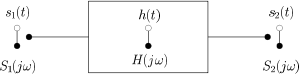
\includegraphics[width=5cm]{./bilder/utf-theorie.png}}\\
\multicolumn{2}{l}{Kaskadierung von wirkungsfreien Systemen:
$H_{total}(s) = H_1(s) H_2(s)$ bzw. bei $n$ gleichen Systemen:
$H_{total} = (H(s))^n$}
 \\ \\

\parbox{13cm}{
	\textbf{Beispiel}: Gesucht UTF $H(s) = \frac{Y(s)}{X(s)}$ \\
	$$H(s) = \frac{sL}{\frac{1}{sC} + sL + R} = \frac{s^2}{\frac{1}{LC} + s
	\frac{R}{L} + s^2}$$\\
	$$\Longrightarrow \text{Pole bei } s = -\frac{R}{2L} \pm j
	\sqrt{\frac{1}{LC} - \left(\frac{R}{2L}\right)^2} \quad ; \quad \text{Doppelte
	Nullstelle bei } s = 0$$
	Differentialgleichung:    $ \ddot{y}(t)+
	\frac{R}{L}\dot{y}(t)+\frac{1}{LC}y=\ddot{x}(t)$}
	
	
	& \parbox{5cm}{
		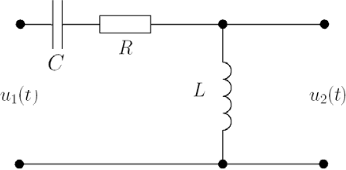
\includegraphics[width=5cm]{./bilder/utf-beispiel.png}} \\
		
\end{tabular}

\subsection{Berechnung des Amplituden- und Phasengangs aus der
Übertragungsfunktion}
$$H(j \omega) = \frac{Y(j \omega)}{X(j \omega)} = \underbrace{|H(j
\omega)|}_{Amplitudengang} e^{j\underbrace{\Theta(\omega)}_{Phasengang}} = 
\frac{|Y(j \omega)|}{|X(j \omega)|} e^{j (\arg(Y(j \omega)) - \arg(X(j
\omega)))} =
\frac{|Y(j \omega)|}{|X(j \omega)|} e^{j \left[\arctan \left(\frac{\Imag\{Y(j
\omega)\}}{\Real\{Y(j \omega)\}} \right) - \arctan \left(\frac{\Imag\{X(j
\omega)\}}{\Real\{X(j \omega)\}} \right)\right]}$$

\subsection{Zusammenhang zwischen Impuls- \& Einheitssprungantwort, Endwerte
\skript{109}}
$ \text{Einheitssprungantwort } g(t) \text{, Impulsantwort }h(t)$
$$h(t)= \frac{\partial g(t)}{\partial t}\quad\text{bzw.}\quad
g(t)=\int_{-\infty}^{t}h(\tau)d\tau \qquad;\qquad 
\lim\limits_{t \rightarrow \infty}  h(t)= \lim\limits_{s \rightarrow 0} s H(s)
\qquad;\qquad
\lim\limits_{t \rightarrow \infty}  g(t)= \lim\limits_{s \rightarrow 0} H(s)$$

\subsection{Phasen- \& Gruppenlaufzeit \skript{116}}
\definecolor{gruppe}{rgb}{1,.75,0} % 255,192,0
\definecolor{phase}{rgb}{1,0,0} % 255,0,0
Die \textcolor{phase}{Phasenlaufzeit}  ist nur für reine Sinussignale bestimmbar:
$\tau_P(\omega)=\frac{-\theta(\omega)}{\omega}$ \\
Die \textcolor{gruppe}{Gruppenlaufzeit} hingegen ist für sämtliche Signale möglich:
$\tau_G(\omega)=\frac{-\partial\theta(\omega)}{\partial\omega}$\\
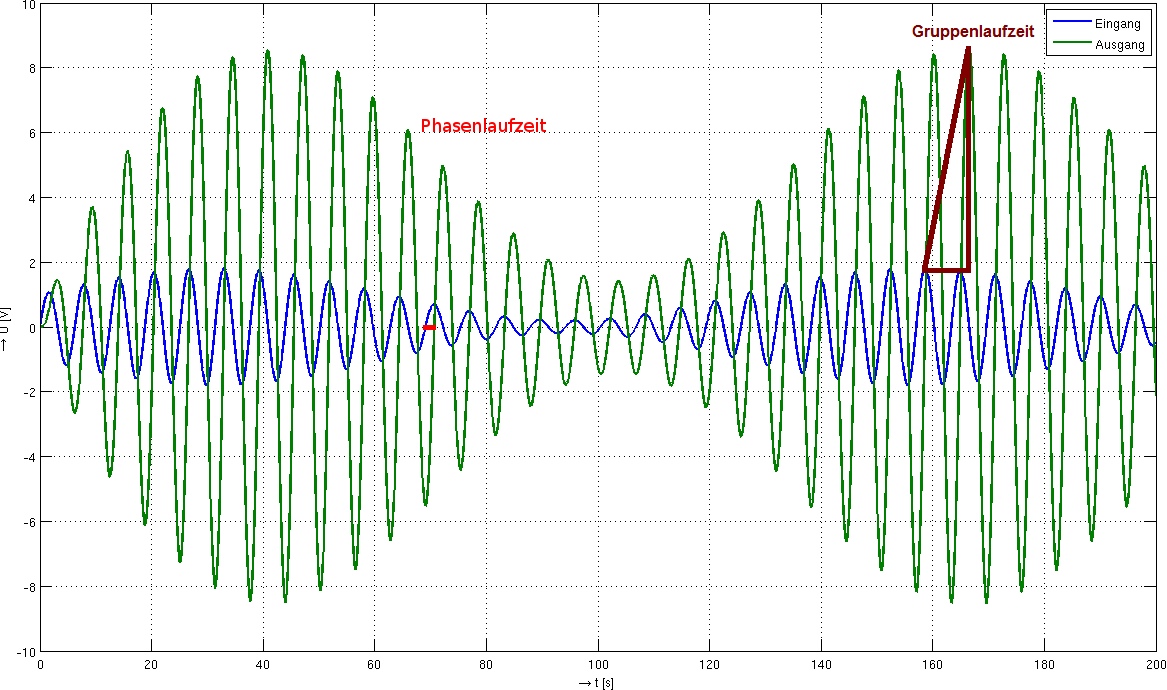
\includegraphics[width=18cm]{./bilder/laufzeit.png}\\
Eingangssignal $x(t)$ und Ausgangssignal $y(t)$ des Systems
$H(s)=\frac{1}{s^2+0.2s+1}$. Bemerkung: $y(t)$ ist gr"osser als $x(t)$.

\subsection{Stabilität von LTI-Systemen}
\subsubsection{Asymptotische Stabilität \skript{112}}
\begin{tabular}{ll}
Stabil: 
	& $\lim\limits_{t\rightarrow\infty} h(t) = 0$ 
	\qquad Pole \textbf{nur} in der
linken s-Halbebene.\\
Instabil: 
	& Mind. ein Pol in der rechten s-Halbebene oder mind. ein
\textbf{mehrfacher} Pol auf der $j$-Achse der s-Ebene. \\
Grenzstabil:
	& mindestens ein \textbf{einfacher Pol} auf der $j$-Achse
\end{tabular}

\subsubsection{Stabilität mit Hurwitz-Polynom \skript{113}}
Es wird jeweils das Polynom im \textbf{Nenner der Übertragungsfunktion} betrachtet:
$P(s) = a_n s^n + a_{n-1} s^{n-1} +\ldots +a_1s + a_0$ \\
\begin{tabular}{|l||l| l|}\hline
$N$   &   $P(s)$ ist ein Hurwitz-Polynom (stabil) &  $P(s)$ ist ein
modifiziertes Hurwitz-Polynom (grenzstabil) \\ \hline\hline
      1     &      gilt f"ur alle $P(s)$          &  $a_0=0$ \\ \hline
      2     &     gilt f"ur alle $P(s)$           &  $a_1=0$ \\ \hline
      3     &     $a_1a_2>a_0a_3$      &  $a_1a_2=a_0a_3$ \\ \hline
      4     &     $a_3(a_1a_2-a_0a_3)>a_1^2a_4$   &    $a_3(a_1a_2-a_0a_3)=a_1^2a_4$\\ \hline

      5    &     {\footnotesize $a_3a_4>a_2a_5$  und}   &     {\footnotesize $a_3a_4>a_2a_5$} \\
           &     {\footnotesize
           $(a_1a_2-a_0a_3)(a_3a_4-a_2a_5)>(a_1a_4-a_0a_5)^2$}   &  
           {\footnotesize $(a_1a_2-a_0a_3)(a_3a_4-a_2a_5)=(a_1a_4-a_0a_5)^2$} 
           \\ \hline   
\end{tabular}\\
\begin{itemize}
  \item Wenn \textbf{ein Koeffizient negativ} ist $(a_x < 0)$, dann ist das System
  \textbf{instabil}.
  \item Wenn \textbf{alle Koeffizienten negativ} sind, kann $-1$ ausgeklammert
  werden und in den Zähler verschoben werden\\ $\Rightarrow$ \textbf{System
  stabil} oder \textbf{grenzstabil} (siehe Punkt 3)
  \item Wenn \textbf{ein Koeffizient nicht vorhanden} ist $(a_x = 0)$, dann ist das System
  evtl. grenzstabil, d.h. es ist eine \textbf{Überprüfung mit modifiziertem Hurwitz-Polynom}
  nötig.
\end{itemize}

\subsection{Klirrfaktor \skript{122}}
Als Mass für nichtlineare Verzerrungen gilt der \textit{Klirrfaktor}. Betrachtet
wird jeweils der Effektivwert am Ausgang 
$$k = \sqrt{\frac{U_2^2 + U_3^2 + \ldots + U_n^2}{U_1^2 + U_2^2 + \ldots +
U_n^2}} \qquad 0 \leq k \leq 1$$ 
\begin{tabular}{ll}
Teilklirrfaktor (frequenzselektiv) 
	&$k_m =  \frac {U_m} {\sqrt{ U_1^2+ U_2^2 + \ldots + U_n^2} }$ \\
Klirrdämpfungsmass 
	& $a_k = 20 \log \left( \frac1k \right)$ $\qquad$ \\
Teilklirrdämpfungmass 
	& $a_k = 20 \log \left( \frac{1}{k_m} \right)$
\end{tabular}

\subsection{Total Harmonic Distortion (THD) \skript{122}}
$$\text{THD} = \sqrt{ \frac {U_2^2+ U_3^2 + \ldots + U_n^2} {U_1^2} } \qquad
\infty > \text{THD} \geq k \geq 0; \quad \text{Für kleine Verzerrungen: THD}
\approx k $$